% Construction (repère mathématique, y vers le haut) :
%   racine 8 en (0, 3) ; 3 en (-2, 2), 10 en (2, 2) ;
%   1 en (-3, 1), 6 en (-1, 1), 14 en (3, 1).
%   Axe du parcours en y = -0.4, chaque clé projetée sur sa propre abscisse.
% SVG : x = 140 + 38x, y = 30 + 38(3 - y).
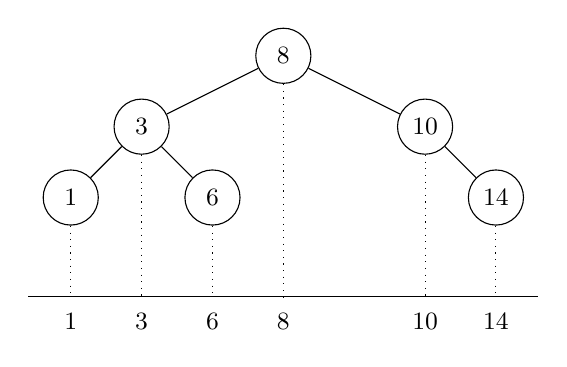
\begin{tikzpicture}[scale=0.9, every node/.style={font=\small}]
  \tikzstyle{cle}=[draw, circle, inner sep=1.5pt, minimum size=7mm]
  \node[cle] (n8)  at (0, 3)  {$8$};
  \node[cle] (n3)  at (-2, 2) {$3$};
  \node[cle] (n10) at (2, 2)  {$10$};
  \node[cle] (n1)  at (-3, 1) {$1$};
  \node[cle] (n6)  at (-1, 1) {$6$};
  \node[cle] (n14) at (3, 1)  {$14$};
  \draw (n8) -- (n3); \draw (n8) -- (n10);
  \draw (n3) -- (n1); \draw (n3) -- (n6); \draw (n10) -- (n14);
  \draw[dotted] (-3, 0.6) -- (-3, -0.4);
  \draw[dotted] (-2, 1.6) -- (-2, -0.4);
  \draw[dotted] (-1, 0.6) -- (-1, -0.4);
  \draw[dotted] (0, 2.6) -- (0, -0.4);
  \draw[dotted] (2, 1.6) -- (2, -0.4);
  \draw[dotted] (3, 0.6) -- (3, -0.4);
  \draw (-3.6, -0.4) -- (3.6, -0.4);
  \foreach \x/\v in {-3/1, -2/3, -1/6, 0/8, 2/10, 3/14}
    \node[below] at (\x, -0.5) {$\v$};
\end{tikzpicture}
